\documentclass{article}
\usepackage{graphicx}
\usepackage{colortbl}
\usepackage{xcolor}
\usepackage{tikz}
\usepackage{booktabs}
\title{\Large\textbf{First-Come First-Served (FCFS) Scheduling Algorithm}}
\author{CPU Scheduler Simulator}
\date{\today}

\begin{document}

\maketitle

\section{Process Details}
FCFS scheduling executes processes in the order of their arrival without preemption.

\begin{table}[h]
\centering
\caption{FCFS Process Scheduling Details}
\label{tab:fcfs_processes}
\begin{tabular}{|c|c|c|c|c|c|c|}
\hline
\textbf{Process ID} & \textbf{Arrival Time} & \textbf{Burst Time} & \textbf{Completion Time} & \textbf{Waiting Time} & \textbf{Response Time} & \textbf{Turnaround Time} \\
\hline
3 & 0 & 3 & 3 & 0 & 0 & 3 \\
\hline
4 & 1 & 3 & 6 & 2 & 2 & 5 \\
\hline
2 & 2 & 4 & 10 & 4 & 4 & 8 \\
\hline
7 & 2 & 7 & 17 & 8 & 8 & 15 \\
\hline
6 & 4 & 1 & 18 & 13 & 13 & 14 \\
\hline
9 & 4 & 1 & 19 & 14 & 14 & 15 \\
\hline
5 & 5 & 10 & 29 & 14 & 14 & 24 \\
\hline
1 & 6 & 7 & 36 & 23 & 23 & 30 \\
\hline
8 & 8 & 8 & 44 & 28 & 28 & 36 \\
\hline
10 & 10 & 8 & 52 & 34 & 34 & 42 \\
\hline
\end{tabular}
\end{table}

\section{Performance Metrics}
The following metrics provide insights into the efficiency of the FCFS scheduling algorithm:

\begin{itemize}
  \item \textbf{Average Waiting Time}: 14.00 time units
  \item \textbf{Average Response Time}: 14.00 time units
  \item \textbf{Average Turnaround Time}: 19.20 time units
  \item \textbf{CPU Utilization}: 100.00\%
\end{itemize}

\textbf{Definitions:}
\begin{itemize}
  \item \textit{Waiting Time}: Time spent waiting in the ready queue
  \item \textit{Response Time}: Time from arrival until first execution
  \item \textit{Turnaround Time}: Total time from arrival to completion
  \item \textit{CPU Utilization}: Percentage of time CPU was busy
\end{itemize}

\section{Gantt Chart}
The Gantt chart below visualizes the execution sequence of processes in FCFS scheduling:

\begin{figure}[h]
\centering
\begin{tikzpicture}[scale=0.7]
\draw[thick] (0,0) -- (53,0);
\draw[thick] (0,0) -- (0,-0.2);
\node at (0,-0.5) {\small 0};
\draw[thick] (5,0) -- (5,-0.2);
\node at (5,-0.5) {\small 5};
\draw[thick] (10,0) -- (10,-0.2);
\node at (10,-0.5) {\small 10};
\draw[thick] (15,0) -- (15,-0.2);
\node at (15,-0.5) {\small 15};
\draw[thick] (20,0) -- (20,-0.2);
\node at (20,-0.5) {\small 20};
\draw[thick] (25,0) -- (25,-0.2);
\node at (25,-0.5) {\small 25};
\draw[thick] (30,0) -- (30,-0.2);
\node at (30,-0.5) {\small 30};
\draw[thick] (35,0) -- (35,-0.2);
\node at (35,-0.5) {\small 35};
\draw[thick] (40,0) -- (40,-0.2);
\node at (40,-0.5) {\small 40};
\draw[thick] (45,0) -- (45,-0.2);
\node at (45,-0.5) {\small 45};
\draw[thick] (50,0) -- (50,-0.2);
\node at (50,-0.5) {\small 50};
\draw[thin] (1,0) -- (1,-0.1);
\draw[thin] (2,0) -- (2,-0.1);
\draw[thin] (3,0) -- (3,-0.1);
\draw[thin] (4,0) -- (4,-0.1);
\draw[thin] (6,0) -- (6,-0.1);
\draw[thin] (7,0) -- (7,-0.1);
\draw[thin] (8,0) -- (8,-0.1);
\draw[thin] (9,0) -- (9,-0.1);
\draw[thin] (11,0) -- (11,-0.1);
\draw[thin] (12,0) -- (12,-0.1);
\draw[thin] (13,0) -- (13,-0.1);
\draw[thin] (14,0) -- (14,-0.1);
\draw[thin] (16,0) -- (16,-0.1);
\draw[thin] (17,0) -- (17,-0.1);
\draw[thin] (18,0) -- (18,-0.1);
\draw[thin] (19,0) -- (19,-0.1);
\draw[thin] (21,0) -- (21,-0.1);
\draw[thin] (22,0) -- (22,-0.1);
\draw[thin] (23,0) -- (23,-0.1);
\draw[thin] (24,0) -- (24,-0.1);
\draw[thin] (26,0) -- (26,-0.1);
\draw[thin] (27,0) -- (27,-0.1);
\draw[thin] (28,0) -- (28,-0.1);
\draw[thin] (29,0) -- (29,-0.1);
\draw[thin] (31,0) -- (31,-0.1);
\draw[thin] (32,0) -- (32,-0.1);
\draw[thin] (33,0) -- (33,-0.1);
\draw[thin] (34,0) -- (34,-0.1);
\draw[thin] (36,0) -- (36,-0.1);
\draw[thin] (37,0) -- (37,-0.1);
\draw[thin] (38,0) -- (38,-0.1);
\draw[thin] (39,0) -- (39,-0.1);
\draw[thin] (41,0) -- (41,-0.1);
\draw[thin] (42,0) -- (42,-0.1);
\draw[thin] (43,0) -- (43,-0.1);
\draw[thin] (44,0) -- (44,-0.1);
\draw[thin] (46,0) -- (46,-0.1);
\draw[thin] (47,0) -- (47,-0.1);
\draw[thin] (48,0) -- (48,-0.1);
\draw[thin] (49,0) -- (49,-0.1);
\draw[thin] (51,0) -- (51,-0.1);
\draw[thin] (52,0) -- (52,-0.1);
\node[draw, thick, fill=orange!40, minimum height=1cm, minimum width=3] at (1.500000,1) {P3};
\node[above] at (0,1.5) {0};
\node[above] at (3,1.5) {3};
\node[draw, thick, fill=pink!40, minimum height=1cm, minimum width=3] at (4.500000,1) {P4};
\node[above] at (6,1.5) {6};
\node[draw, thick, fill=green!40, minimum height=1cm, minimum width=4] at (8.000000,1) {P2};
\node[above] at (10,1.5) {10};
\node[draw, thick, fill=red!40, minimum height=1cm, minimum width=7] at (13.500000,1) {P7};
\node[above] at (17,1.5) {17};
\node[draw, thick, fill=blue!40, minimum height=1cm, minimum width=1] at (17.500000,1) {P6};
\node[above] at (18,1.5) {18};
\node[draw, thick, fill=yellow!40, minimum height=1cm, minimum width=1] at (18.500000,1) {P9};
\node[above] at (19,1.5) {19};
\node[draw, thick, fill=purple!40, minimum height=1cm, minimum width=10] at (24.000000,1) {P5};
\node[above] at (29,1.5) {29};
\node[draw, thick, fill=yellow!40, minimum height=1cm, minimum width=7] at (32.500000,1) {P1};
\node[above] at (36,1.5) {36};
\node[draw, thick, fill=cyan!40, minimum height=1cm, minimum width=8] at (40.000000,1) {P8};
\node[above] at (44,1.5) {44};
\node[draw, thick, fill=green!40, minimum height=1cm, minimum width=8] at (48.000000,1) {P10};
\node[above] at (52,1.5) {52};
\begin{scope}[yshift=-2cm]
\node[draw, thick, fill=gray!20, minimum height=0.5cm, minimum width=1cm] at (1,0) {};
\node[right] at (1.7,0) {Idle time};
\node[draw, thick, fill=cyan!40, minimum height=0.5cm, minimum width=1cm] at (6,0) {};
\node[right] at (6.700000,0) {Process P0};
\node[draw, thick, fill=yellow!40, minimum height=0.5cm, minimum width=1cm] at (10,0) {};
\node[right] at (10.700000,0) {Process P1};
\node[draw, thick, fill=green!40, minimum height=0.5cm, minimum width=1cm] at (14,0) {};
\node[right] at (14.700000,0) {Process P2};
\node[draw, thick, fill=orange!40, minimum height=0.5cm, minimum width=1cm] at (18,0) {};
\node[right] at (18.700000,0) {Process P3};
\node[draw, thick, fill=pink!40, minimum height=0.5cm, minimum width=1cm] at (22,0) {};
\node[right] at (22.700000,0) {Process P4};
\node[draw, thick, fill=purple!40, minimum height=0.5cm, minimum width=1cm] at (26,0) {};
\node[right] at (26.700000,0) {Process P5};
\node[draw, thick, fill=blue!40, minimum height=0.5cm, minimum width=1cm] at (30,0) {};
\node[right] at (30.700000,0) {Process P6};
\node[draw, thick, fill=red!40, minimum height=0.5cm, minimum width=1cm] at (34,0) {};
\node[right] at (34.700000,0) {Process P7};
\end{scope}
\end{tikzpicture}
\caption{FCFS Scheduling Gantt Chart}
\label{fig:fcfs_gantt}
\end{figure}

\section{Conclusion}
First-Come First-Served (FCFS) is the simplest CPU scheduling algorithm, where processes are executed in the order they arrive in the ready queue. Key characteristics of FCFS include:

\begin{itemize}
  \item Non-preemptive scheduling (once a process starts, it runs to completion)
  \item Simple to implement and understand
  \item Can suffer from the ''convoy effect'' where short processes wait behind long ones
  \item Average waiting time is often not minimal compared to other algorithms
\end{itemize}

\end{document}
